% !TEX root = creche.tex
\documentclass[creche.tex]{subfiles}
\begin{document}
\chapter*{Preface}
\addcontentsline{toc}{chapter}{Preface}
\label{praface}
\vspace*{-8ex}
\hfill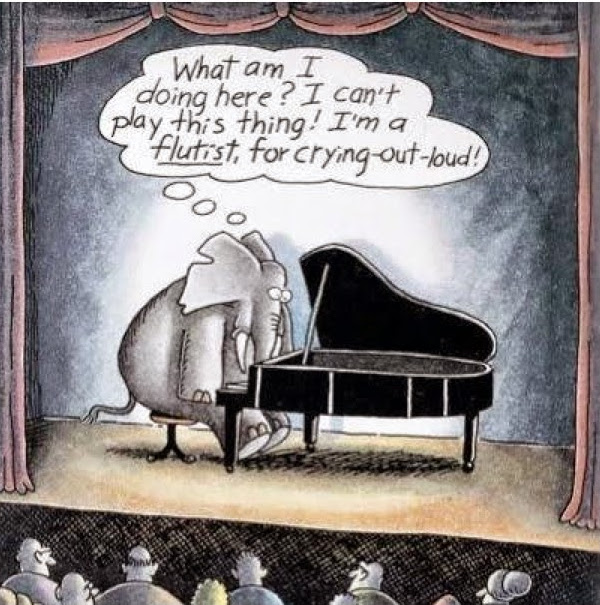
\includegraphics[width=.4\textwidth]{elephant_playing_piano.jpg}


\vspace*{-22ex}
\begin{minipage}{0.58\textwidth}
These are the notes of a course that I have been giving for a few years in Amsterdam and many more in Turin. A few chapters are missing and will be added soon. I keep the most recent version in

\smallskip
\href{github.com/domenicozambella/creche}{https://github.com/domenicozambella/creche}
\smallskip

Below I list a few peculiarities of the exposition.
\end{minipage}

\vskip5ex


\begin{itemize}
\item \hyperref[rich]{Fraïssé limits} are presented in a slightly general setting which accommodates more examples (and I'll add a few more). This is used e.g.\@ to discuss saturation.
\item \hyperref[algebraic]{Quantifier elimination for ACF} and Hilbert's Nullstellensatz are presented with more details than usual. (This annoys most of the readers. Still, I hope it may help some students.)
\item The proof of the \hyperref[countable]{Omitting Types Theorem} uses a model theoretic construction (different from the standard syntactic proof).
\item \hyperref[imaginary]{Imaginaries and the eq-expansion} are introduced from the (equivalent) dual perspective: the canonical name of a definable set is the set itself.
\item \hyperref[Ramsey]{Ramsey Theorem} is derived from the existence of coheir sequences. Admittedly, this is not the shortest proof, but it may be interesting. I plan to add a proof of Hindman's theorem along the same lines.
\item \hyperref[invariantL]{Lascar and Kim-Pillay types} are introduced in a slightly unconventional way. I am grateful to Krzysztof Krupiński for helping me squaring the circle with KP-types.
\item \hyperref[newelski]{Newelski's Theorem\/} on the diameter of Lascar types is proved in an elementary self-contained way.
\end{itemize}
\end{document}
